
The Open Global Glacier Model (OGGM) is an open source modelling framework for glaciers. It has been developed since
2014: intermittently at first, and more regularly since 2016. Today, OGGM is continuously discussed and updated by a
team of researchers in various institutions.

“OGGM e.V” is a registered non-profit organization, which purpose is the promotion of science and research in the fields
of climate and glaciology; it does so by coordinating the development of OGGM and OGGM-Edu, and by organizing events
around the topic of large-scale glaciology.
\begin{itemize}
\item {} 
\textbf{Website:} \href{https://oggm.org}{https://oggm.org}

\item {} 
\textbf{Model documentation:} \href{http://docs.oggm.org}{http://docs.oggm.org}

\item {} 
\textbf{Online tutorials:} \href{http://oggm.org/tutorials}{http://oggm.org/tutorials}

\item {} 
\textbf{Source code:} \href{https://github.com/OGGM/oggm}{https://github.com/OGGM/oggm}

\item {} 
\textbf{Social media (twitter):} \href{https://twitter.com/OGGM\_org}{https://twitter.com/OGGM\_org}

\end{itemize}

Anyone can participate in the development of OGGM. In practice, however, the main bulk of development and funding effort
in the past have come from the Universities of Bremen (Ben Marzeion) and Innsbruck (myself). I have contributed to the
vast majority of the codebase, while strategic decisions have been shared between Ben and me, and in recent years with a
growing community of users.

This chapter briefly describes the OGGM project, its mission and building blocks. It concludes with a discussion about
some of the challenges the project is facing. For a discussion about the project’s future and long-term perspectives,
refer to Sect.~\ref{perspectives}.


\section{Objectives of the OGGM project}

The main mission of the OGGM project is to:

\begin{quote}
Develop a \textbf{global scale}, \textbf{modular}, and \textbf{open source} numerical model framework for \textbf{consistently} simulating past and future global scale glacier change
\end{quote}

\textbf{Global scale} means that OGGM should be applicable to all the world glaciers. This also means that it should be
applicable to a smaller ensemble of glaciers, for example at the catchment scale, or even one single glacier. However,
OGGM’s main added value will always be its ease of use and applicability to large numbers: this means that it is
acceptable for us that OGGM is less useful or accurate at the single glacier scale than other methods would.

\textbf{Modular} means that we want OGGM to allow for different modelling approaches, for example different representations
of ice flow or of the surface mass balance. Although we have to pick a default modelling workflow for the model to
work “out of the box”, we do not want to enforce it. This has long been misunderstood outside the OGGM community, and
in recent years we have put more effort in re-branding OGGM as a “modelling framework” rather than a model alone. The
importance of modularity for running model intercomparison experiments is discussed below.

\textbf{Open source} means that code can be read and used by anyone so that new modules can be added and discussed by the
community. OGGM’s permissive license allows any individual or entity to use it without any restriction. It also means
that we will always put a lot of effort on code documentation and testing: indeed, very much like data without metadata,
code without a documentation is practically useless.

\textbf{Consistency} relates to all three points raised above. Consistency in the modelling chain (regardless of the glacier
or region it is applied to) allows providing uncertainty measures at all realizable scales (in theory - in practice
this is quite complex). Consistency combined with modularity allows running sensitivity experiments with fixed and well
controlled boundary conditions: it allows isolating specifically for the influence of a parameterization choice rather
than a suite of modelling decisions. Consistency in the context of open-source development means that a fixed OGGM
version should always produce the same results, regardless of the computer and operating system that was used to run it.
It also means that differences between OGGM versions should be documented and that older OGGM versions should be
permanently archived.


\subsection*{Project non-goals}

Our project does not aim to make of OGGM the single venue for future regional or global glaciological studies. We
strongly believe in the usefulness of model inter-comparisons and on the necessity to have various ways to solve the
same problem, for the sake of scientific repeatability and replicability. “Healthy” competition drives innovation.

However, we attempt to encourage model developers to make their model operable within the OGGM workflow, while still
keeping their model’s specificities, name, code, etc. under their full control and outside the OGGM namespace. We
believe that this will greatly facilitate the standardization and execution of future model inter-comparisons.


\section{Fundamental concepts}

I briefly summarize the model’s building blocks: not to be comprehensive, but to give enough of an overview for the
readers to understand the discussions that will follow. For a more in-depth introduction, refer to
Paper 01 or the \href{http://docs.oggm.org}{model documentation}.


\subsection{Glacier centric model}


OGGM is what we called a “glacier centric model”, which means that it runs for each glacier independently of the
others. In the case of glacier complexes, it relies on the glacier inventory to properly separate the individual glacier
entities by the ice divides, ensuring that all ice in a glacier basin flows towards a single glacier terminus (this is
unfortunately not always the case).

\begin{figure}[h]
\centering
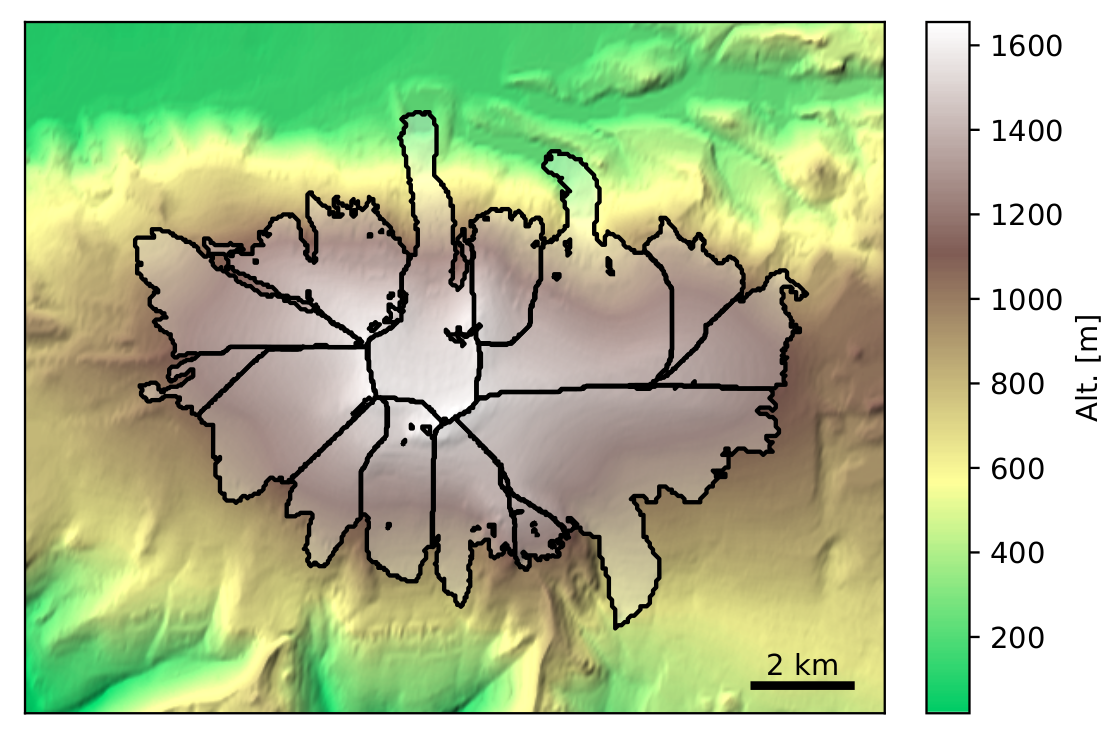
\includegraphics[width=0.7\linewidth]{\figs/iceland.png}
\caption{Glacier centric approach applied to the Eyjafjallajökull ice cap in Iceland.  Glacier outlines provided by the Randolph Glacier Inventory v6.0.}
\end{figure}

The glacier centric approach is used by most large-scale glacier models to date. Alternative strategies include global
gridded approaches \citep{Shannon2019}, where all glaciers in a model grid cell are added together and possibly
organized into elevation bins. Another approach is to handle entire glacier complexes as one single body of ice (“ice
caps”). This is physically consistent and feasible, but requires either distributed models of ice flow
\citep{Furst2017} (computationally expensive) or implies simplifications to the glacier geometry (so that all ice flows
downwards, \citep{Huss2012}).

The advantage of glacier centric models is their adherence to the de-facto standard inventory of glacier outlines:
the \href{https://www.glims.org/RGI/}{Randolph Glacier Inventory}. Any glacier can be selected and simulated, and the model
output can be compared to standard reference datasets such as length changes or surface mass balance data from
the \href{https://wgms.ch}{World Glacier Monitoring Service}. Various models can be compared on a glacier per glacier basis
or a combination of them. It is also computationally efficient, since models can focus on simulating the areas where
glaciers are really located. This may sound trivial, but glacier centric models can also make use of the glacier
location as a boundary condition, e.g. by excluding unrealistic solutions to the problem of computing mass balance or
inferring ice thickness, for example.

The disadvantage of glacier centric models is their questionable scientific validity in presence of glacier complexes
and ice divides (this problem can be mitigated by defining glacier complexes as one single entity, requiring other
strategies than currently standard in OGGM). A larger issue of glacier centric models is that they are focussed on
simulating glaciers that have been inventoried, i.e. they cannot retrieve past (or present) uncharted glaciers
\citep{Parkes2018}. For these reasons, they are not well adapted for studying glacier evolution in climates when
glaciers were widely different from today (e.g. the Last Glacial Maximum).


\subsection{Standard modelling workflow}

I briefly illustrate the OGGM workflow with an example application on the Tasman Glacier in New Zealand (see figure
below). Refer to the model documentation for more information.

\textbf{Preprocessing.}
The glacier outlines are extracted from a reference dataset (RGI)
and projected onto a local gridded map of the glacier (Fig.~\ref{fig:flow}a). Depending on the glacier location, a suitable source
for the topographical data is downloaded automatically and interpolated to the local grid. The spatial resolution of the
map depends on the size of the glacier.

\textbf{Flowlines.}
The glacier centerlines are computed using a geometrical routing algorithm
(Fig.~\ref{fig:flow}b), then filtered and slightly modified to become glacier “flowlines”
with a fixed grid spacing (Fig.~\ref{fig:flow}c).

\textbf{Catchment areas and widths.}
The geometrical widths along the flowlines are obtained by intersecting the normals at each grid point with the glacier
outlines and the tributaries’ catchment areas. Each tributary and the main flowline has a catchment area, which is then
used to correct the geometrical widths so that the flowline representation of the glacier is in close accordance with
the actual altitude-area distribution of the glacier (Fig.~\ref{fig:flow}d).

\textbf{Climate data and mass balance.}
Gridded climate data (monthly temperature and precipitation) are interpolated to the glacier location and corrected for
the altitude at each flowline’s grid point. A calibrated mass balance model is used to compute the mass balance for the
past, and for projections based on GCM data.

\textbf{Ice thickness inversion.}
Using the mass balance data computed above and relying on mass-conservation considerations, an estimate of the ice flux
along each glacier grid point cross-section is computed by making assumptions about the shape of the cross-section.
Using the physics of ice flow and the shallow ice approximation, the model then computes the thickness of the glacier
along the flowlines and the total volume of the glacier (Fig.~\ref{fig:flow}e).

\textbf{Glacier evolution.}
A dynamical flowline model is used to simulate the advance and retreat of the glacier under preselected climate time
series. Here (Fig.~\ref{fig:flow}f), a 120-yrs long random climate sequence leads to a glacier advance.


\begin{figure}[h]
\centering
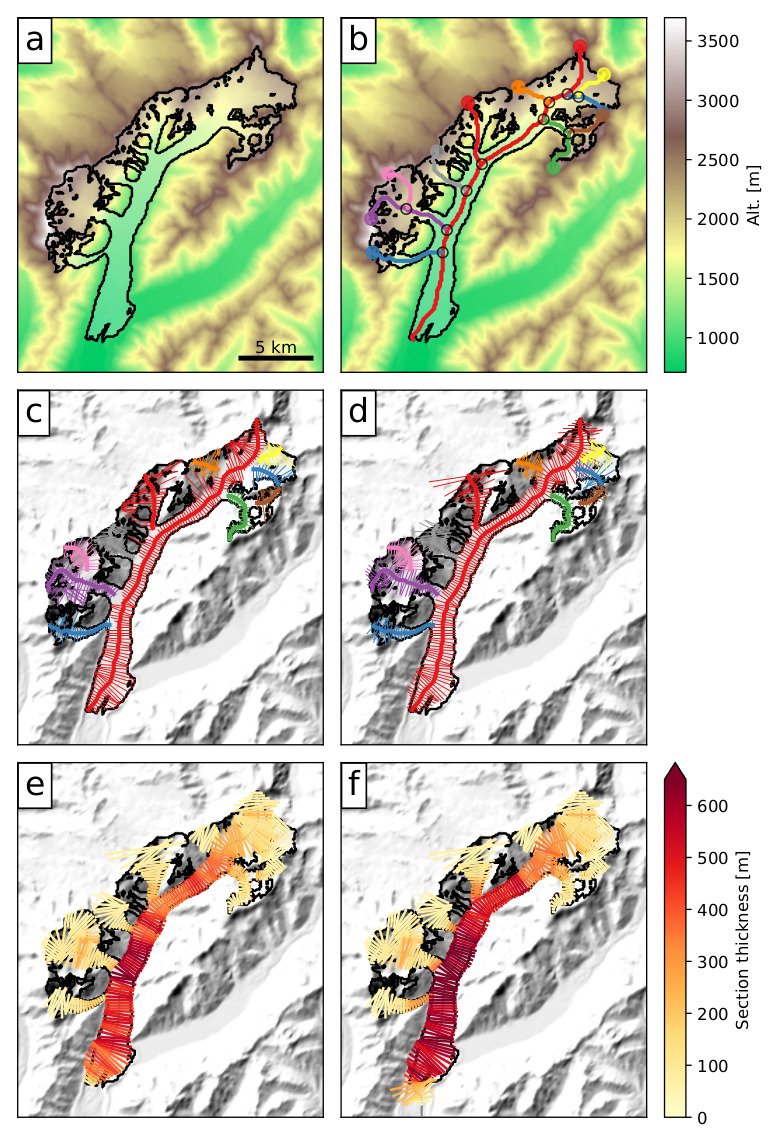
\includegraphics[width=0.700\linewidth]{\figs/ex_workflow.png}
\caption{Illustration of the OGGM standard workflow applied to Tasman Glacier.}
\label{fig:flow}
\end{figure}


\subsection{OGGM data structures and glacier directories}

The fundamental data structure used in OGGM is the so-called \textbf{Glacier Directory}. Glacier directories simply are
folders on disk which store the input and output data for a single glacier during a run. OGGM offers an object interface
to access and store these files programmatically.

This very simple idea is at the core of the OGGM workflow: actions to perform on glaciers (“tasks”, see below) are given
access to the data files via the glacier directory interface, read data they need from disk, and write back to it.

This design matches perfectly the “glacier centric” modelling strategy, and has many advantages:
\begin{itemize}
\item {} 
there is no practical difference between simulating one single, or many glaciers: all glacier directories are
independent of another.

\item {} 
data is persistent on disk: workflows can be interrupted and restarted from disk at no cost overhead. Workflows can
even be prepared on one computer and restarted from another computer (see example below).

\item {} 
“modularity” is achieved via data formats, not via programmatic interfaces: various ways to compute the flowlines (for
example) can co-exist if they agree on how a flowline is stored on disk.

\item {} 
multiprocessing is trivial: the same task can be run on many glaciers at once without having to share data across
processes, since everything is on disk and independant.

\end{itemize}

This persistence en disk has a few drawbacks as well:
\begin{itemize}
\item {} 
for the glacier directories to be independent, several data sources are duplicated: topography for example (each
glacier has its own subset of the original data, often overlapping with neighbors), or climate timeseries (the same
data from the same grid point is stored in various directories). This can lead to rather large data storage
requirements, but can be mitigated by deleting intermediate files.

\item {} 
since users can restart workflows from pre-processed states, the code that was used to produce them is often ignored
or might be older, etc. This can lead to silent bugs (for example mismatching model parameters between the preprocessing
and the simulations, leading to incorrect results). Because of this issue, we had to implement safeguards against such
mistakes where possible.

\item {} 
users can be confused by glacier directories. Since an OGGM program does not always read like linear “A to Z”
workflows (but for example “start from Q, then Q to Z”), mistakes like the ones described above can happen unnoticed.

\item {} 
it can make certain types of sensitivity experiments more difficult to implement, since users not only have to care
about variable names, but also data file names.

\end{itemize}

Here is an example of how glacier directories work in practice. The user indicates a repository from which
they want to fetch the data, and a list of glacier IDs they’d like to start from. The \mintinline{python}{init_glacier_directories}
performs the action of downloading and extracting these data locally.

\begin{figure}[H]
\captionsetup{singlelinecheck = false, justification=justified} 
\begin{minted}
[
]
{python}
from oggm import workflow, graphics

# Glaciers to simulate
rgi_ids = ['RGI60-11.01328', 'RGI60-11.00897']
# Where to fetch the pre-processed directories - this can be changed
server_url = 'https://cluster.klima.uni-bremen.de/~oggm/gdirs/'
experiment_url = 'oggm_v1.4/L3-L5_files/CRU/centerlines/qc3/pcp2.5/no_match'
base_url = server_url + experiment_url
# Fetch them
gdirs = workflow.init_glacier_directories(rgi_ids, from_prepro_level=3, 
                                          prepro_base_url=base_url)
# Plot the ice thickness inversion results
graphics.plot_inversion(gdirs[0])
\end{minted}
\vspace{10mm}
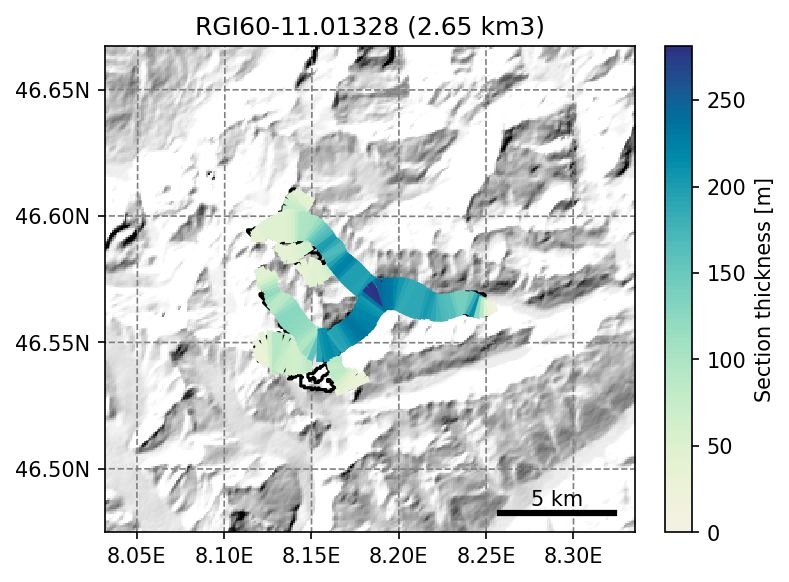
\includegraphics[width=0.600\linewidth]{\figs/unteraar_demo.png}
\caption{Example of the glacier directory workflow}
\end{figure}

See also the documentation page for \href{https://docs.oggm.org/en/stable/input-data.html}{OGGM-Shop}
for more examples of the kind of data that can be added to glacier directories.


\subsection{OGGM tasks}

Tasks in OGGM are actions to perform on one single glacier (“entity tasks”) or several of them (“global tasks”). Tasks
have a special meaning in the OGGM workflow and are applied as such:

\begin{figure}[H]
\begin{minted}
[
]
{python}
# Initialize glacier dir
from oggm import workflow, tasks

ectories
gdirs = workflow.init_glacier_directories(rgi_ids)

# Define the list of tasks
task_list = [
    tasks.define_glacier_region,
    tasks.glacier_masks,
    tasks.compute_centerlines,
    tasks.catchment_area,
    tasks.catchment_width_geom,
]

# Apply them sequentially
for task in task_list:
    workflow.execute_entity_task(task, gdirs)
\end{minted}
\end{figure}


\mintinline{python}{exectute_entity_task} will apply the given task to a list of glaciers. If multiprocessing is switched on, all glaciers
will be processed in parallel, making full use of all available processors. Here we apply the default tasks with default
settings, but parameters can be changed via global settings or function arguments.

Depending on the desired set-up, tasks can be replaced by others (e.g. the centerlines tasks can be replaced by other
algorithms) or omitted (for example, users can choose whether a quality check filter should be applied to the climate
timeseries or not).


\begin{figure}[h]
\centering
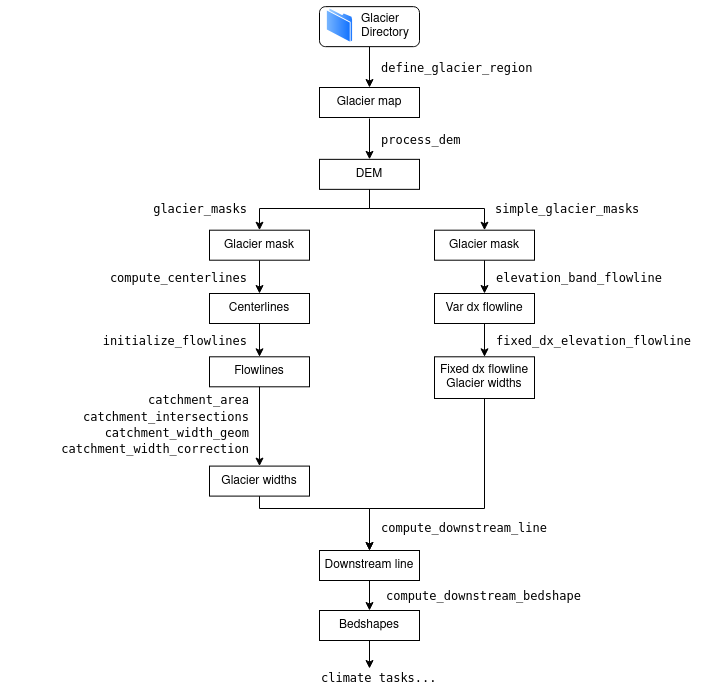
\includegraphics[width=0.700\linewidth]{\figs/flowchart_flowlines.png}
\caption{Example flowchart illustrating how OGGM implemented support for two kinds
of flowline representations for a glacier: centerlines on the left (OGGM’s default)
and binned elevation bands flowlines on the right (after \citet{Huss2012}).}
\end{figure}

\subsection{Take home messages}

The purpose of this rather technical description was to convey the general design of the model around the concept of a
list of tasks to be applied to glacier entities and that store their output in glacier directories on disk. Note that
except for their names and the objects they are referring to (glaciers), these “building blocks” are largely
agnostic to the kind of tasks that have to be applied, and I deliberately did not provide any modelling detail here.

This is important, because I believe that the OGGM project should not be considered by looking only at the physics
choices we’ve made for each of these tasks or their default parameters. OGGM should also be evaluated for the new
developments its structure can allow. OGGM does not enforce a particular modelling strategy beyond the constraints
defined above: in summary, complying models do need to follow the glacier directory approach (otherwise OGGM will be of
very little use for them). If new modelling groups develop ideas based on a glacier centric approach, they can make use
of OGGM’s building blocks and add their own, provided that they comply with this “OGGM way of doing things”.

By doing so, external projects based on OGGM will then benefit from all future developments in OGGM, and the other way
around: OGGM can then use and apply these external modules. If desired, external projects can also benefit from the
suite of modern open development tools that OGGM provides. I describe them below.


\section{Open development practices}

OGGM development has been strongly inspired by practices which have become a standard in the software development
community, but that are (unfortunately) not yet well known in the scientific community.

Like the vast majority of today’s software, OGGM’s development is done under a version control system
called \href{https://git-scm.com/}{git}. The OGGM repository is hosted on \href{https://github.com/OGGM/oggm}{github}, enabling
many of the tools described below.


\subsection{Code review}

Very much like peer-review, open development practices based on git enable code review. Open code review has many
advantages:
\begin{itemize}
\item {} 
it gives model developers the opportunity to discuss changes alongside the code rather than per email

\item {} 
it improves code quality, since more than one person can look at the code

\item {} 
it gives an opportunity to model users to follow changes in the model even if they are not actively participating

\item {} 
code changes and associated comments over time are stored online for later reference

\end{itemize}


\begin{figure}[h]
\centering
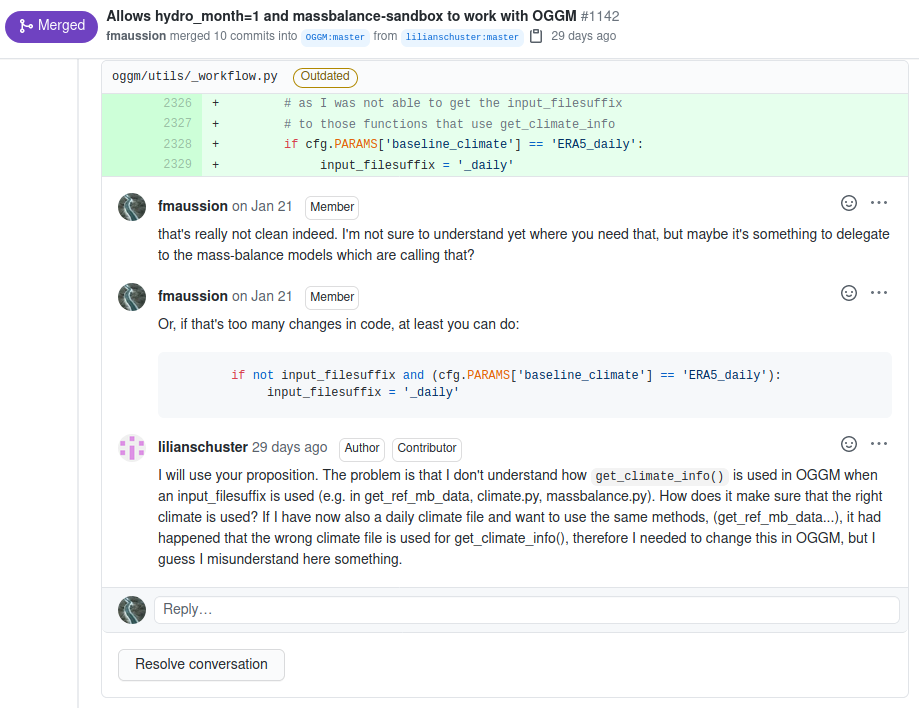
\includegraphics[width=0.900\linewidth]{\figs/pr.png}
\caption{Example of code review in a recent “\href{https://github.com/OGGM/oggm/pull/1142}{pull-request}”.}
\end{figure}

Ideally, all code submissions to OGGM should be peer-reviewed. In practice, however, only the contributions from others
than me are reviewed (by me). I’ll discuss this problem in more length below.


\subsection{Testing strategy}

OGGM enforces a strict code testing strategy: all additions to the code must be supplemented by appropriate tests. The
tests have the purpose to check that the code (i) can be executed without errors and (ii) works as expected. These tests
are an integral part of the codebase, and all of them are run each time a new code addition is suggested (a process
called \href{https://en.wikipedia.org/wiki/Continuous\_integration\#Run\_tests\_in\_CI}{continuous integration}), hereby
avoiding “regressions” as much as possible (when a change in one part of the code affects another in non-predictable
ways).

\begin{figure}[h]
\centering
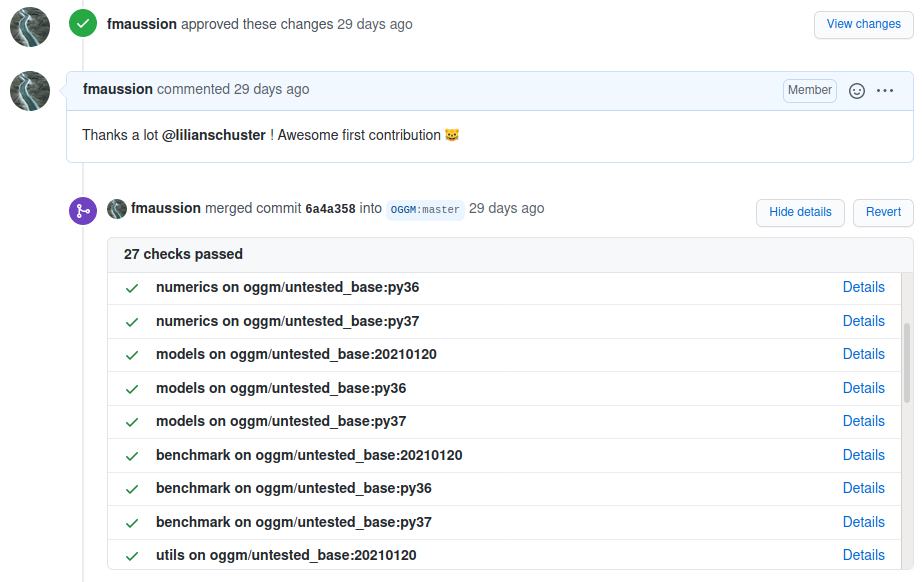
\includegraphics[width=0.700\linewidth]{\figs/tests.png}
\caption{Example of automated testing in a recent “\href{https://github.com/OGGM/oggm/pull/1142}{pull-request}”.}
\end{figure}


\subsection{Online documentation and tutorials}

Making code available is, by far, not enough to make code accessible. As of today, the OGGM codebase contains several
thousands of lines of code, making it very difficult for anyone new to the project to understand the model’s structure
just by reading the code.

Lack of code documentation (and the high cost of writing documentation) is probably one of the main obstacles towards
more open code sharing practices, as many scientists do not feel comfortable to share undocumented code. OGGM is no
exception (I always feel there could be better documentation for almost everything), but thanks to a suite of great
open-source tools, writing documentation for OGGM can also be rewarding. Writing documentation is also a very good way
to engage the community of users towards OGGM’s development, since contributing to the documentation can feel easier
than contributing to the code.

OGGM’s documentation relies on three main elements:
\begin{enumerate}

\item {} 
The project website (\href{https://oggm.org}{https://oggm.org}) for general, non code related project communication and blog posts.

\item {} 
The technical documentation (\href{https://docs.oggm.org}{https://docs.oggm.org}) to document model physics, model structure, and function calls
definitions.

\item {} 
The tutorials (\href{https://oggm.org/tutorials}{https://oggm.org/tutorials}) with hands-on model applications in various use cases.

\end{enumerate}

The project website is built using \href{https://jekyllrb.com/}{jekyll}, a static site generator. It’s source code and
content is also open and stored \href{https://github.com/OGGM/oggm.github.io}{on github}.

The technical documentation is built using \href{https://www.sphinx-doc.org}{sphinx} and is hosted
on \href{https://readthedocs.org/}{readthedocs}. Its content is stored alongside the code on the main repository.

The tutorials are written with \href{https://en.wikipedia.org/wiki/Project\_Jupyter\#Jupyter\_Notebook}{Jupyter Notebooks} and
rendered online with \href{https://jupyterbook.org}{Jupyter-Book}. The notebook interface allows sharing text and formulas
alongside the code, making them particularly adapted for tutorials. In addition, tutorials can be run and explored
interactively thanks to \href{https://mybinder.org}{MyBinder}. This is a great tool to engage new users, since they can try
the model online before going the struggle of installing it.


\subsection{Reproducibility}

OGGM attempts to make results obtained with the
model \href{https://en.wikipedia.org/wiki/Reproducibility\#Reproducible\_research}{reproducible} as far as possible. To do so,
the OGGM stable versions are stored with a DOI on \href{https://zenodo.org/record/4546676}{Zenodo}, and authors
are \href{https://docs.oggm.org/en/stable/citing-oggm.html}{encouraged} to use and cite stable OGGM versions (we can also
store older versions on demand if necessary).

Furthermore, a central tool that we offer to ensure that OGGM results are reproducible no matter the machine it is
running on, or the version of software packages that are installed
are \href{https://docs.oggm.org/en/stable/practicalities.html\#singularity-and-docker-containers}{docker containers}.
Containers are like a “software capsule”: they contain everything that OGGM needs to run and can be executed by any
machine that has Docker installed.


\section{Challenges}

To my knowledge at the time of writing, OGGM has been used for at least 13 peer-reviewed publications (3 are in review)
and has been an important part of 3 completed PhD theses. We expect these numbers to grow in the future, with new
generations of students and new collaborations starting just now. Several other indicators are suggesting that the OGGM project is being used by other
research groups, such as the number of requests to join our discussion channels and to use OGGM-Hub.

The fact that the OGGM project is now expected to suit these various needs
(new users with various expectations about OGGM capabilities, PhD students and PostDocs under time pressure,
project deadlines, etc) comes with a number of challenges which I briefly describe here.


\subsection{Technical debt}

The OGGM code base has grown and continues to grow organically, at the pace at which new features are added to the
model. Future innovation will be slowed down and maybe even impeded by the so-called “technical debt”: code that works
but would need considerable refactoring to adapt to new ideas and to allow further development.

Accumulating technical debt also makes testing the software and ensuring the validity of its results more challenging.
Certain functions might have been written in the past to take into account situations which are no longer an issue
today, adding unnecessary complexity to the code.

This often needed refactoring (process of restructuring and modernizing existing computer code)
is not without costs: it takes considerable time, is not rewarded by traditional academic measures such as publications,
and needs to be carefully conducted in order not to introduce new bugs into the software. Perhaps even more
problematically: existing users who wrote code based on OGGM are very unwilling to update it to the new OGGM versions (I
know this from experience).

There is therefore a trade-off between breaking backwards compatibility (i.e. breaking existing code) and
innovating. Other models with fewer users, or lower standards in terms of code reusability (this is not always a bad thing),
may be more agile and quicker in innovating because no other people are relying on their code being stable.


\subsection{Software maintenance and entry level for new contributors}

A large part of routine software development maintenance currently relies on one or two main developers (myself, and an
IT technician in Bremen who is in charge of the technical aspects of the deployment of OGGM).
This work takes a lot of time (mainly because every new feature needs to be tested and documented), and my time is
limited. Therefore, the development process is slower than I’d like it to be.

As the software grows and increases in complexity, it becomes more difficult for new users to understand the model’s
structure and to apply it to their specific research problem. Furthermore, it makes it harder for new users to
envision a potential contribution to the code base. The typical model contributors (PhD students and post docs) are
employed on fixed-term contracts, causing a high turnover, making transmission of knowledge particularly difficult.

Finally, not all scientists are interested in writing reusable code, as is required when contributing to OGGM.
Very few have the time, energy, or interest to invest in the rather demanding field of scientific programming,
while staying on top of the other requirements of our job. I had the privilege to be given enough time to realize this
project over the course of several years, thanks to my stable employment at the university of Innsbruck. No other
traditional funding scheme in Austria would have allowed this kind of long haul development work.

The future of OGGM’s technical development and maintenance therefore strongly relies on funding agencies
acknowledging that open-source development work is an integral part of the scientific process. Employers should reward
open source work at the same level as scientific publications when considering applications.


\subsection{Innovation with OGGM}

I often ask myself the question of the role of OGGM in comparison to similar models in the geosciences.
Let’s take the atmospheric model \href{https://www.mmm.ucar.edu/weather-research-and-forecasting-model}{WRF}
as a prominent example. WRF is open-source, and its user base is obviously larger than OGGM by several orders of
magnitude. The reason is not only that WRF is an atmospheric model, and a much more mature and feature complete model.
I believe that a major reason is that users can take the model, learn how to use it (without knowing the internal
details of its functioning), and apply it to their research question with very few modifications (change of domain,
change of boundary conditions).

Attempting to make a parallel with OGGM will unravel some differences:

\begin{itemize}
\item {} 
For one, OGGM already simulates
all glaciers. I.e. “changing the domain” is not meaningful, unless the study attempts to simulate glaciers
differently, or analyse the data from a new perspective.

\item {} 
Second, since OGGM is highly parameterized, applying it blindly, without a specific awareness of its simplifications
and potential pitfalls, is not recommended.
This point is also valid for WRF, but I would argue that it is less problematic: thanks to the large
amount of available data for independent validation, users are able to check if their simulations are meaningful.
With a model like WRF, where the boundaries between calibration and validation data are fuzzier, it is difficult
for users to assess whether they apply the model correctly or not.

\item {} 
Finally, application of OGGM to a new research question almost inevitably leads to the development of extensions to
OGGM, or modifications of its internal code. This comes with the nature of the model: since the standard modelling of all
glaciers is possible “out-of-the box”, innovation can only come with active participation in the model development,
it’s capacity to deal with new boundary conditions, a new model parameterization, etc.

\end{itemize}

To summarize, and despite all our efforts to make OGGM user-friendly, I think that for the time being OGGM is
still a model “for modellers”, not yet ready for blind application. Because of the nature of the problems that
OGGM is trying to solve, it might never be “a model for users”, and remain “a model (or framework) for modellers”.
I think that this is something I’d be happy with, but it has implications for the people willing to learn how to apply
the model -- in particular in terms of required programming and glacier modelling skills.